\documentclass[xcolor=dvipsnames,aspectratio=169]{beamer}

% INCLUSIÓN DOS PAQUETES IMPRESCINDIBLES DE IDIOMA E CODIFICACIÓN DE CARACTERE.
\usepackage[T1]{fontenc}
\usepackage[english]{babel}
\usepackage[utf8]{inputenc}
\usepackage{csquotes}

%ACRONYMS para engadir un glosario de acronimos automatizado
% \usepackage[acronyms,nonumberlist,nopostdot,nomain,nogroupskip]{glossaries}
% \input{./acronyms.tex}

% PAQUETES PARA FIGURAS E GRAFICOS
\usepackage{graphicx}
%   \usepackage[pdftex]{graphicx}
  \usepackage{epstopdf}
   \graphicspath{{./img/}}
  % and their extensions so you won't have to specify these with
  % every instance of \includegraphics
   \DeclareGraphicsExtensions{.eps,.pdf,.png,.jpg}   
\usepackage{subfigure}
\usepackage{caption}

%Tikz plots
\usepackage{tikz}
\usepackage{tikzscale}
\usetikzlibrary{plotmarks,patterns,decorations.pathreplacing,backgrounds,calc,arrows,arrows.meta,spy,matrix,backgrounds,shapes}

\tikzset{
    block/.style = {draw, rectangle, 
        minimum height=1cm, 
        minimum width=1.2cm},
    input/.style = {coordinate,node distance=1cm},
    output/.style = {coordinate,node distance=2cm},
    arrow/.style={draw, -latex,node distance=1.5cm},
    pinstyle/.style = {pin edge={latex-, black,node distance=1.5cm}},
    sum/.style = {draw, circle, node distance=1cm}
}
\newcommand{\tikzmark}[1]{\tikz[overlay,remember picture] \UE (#1) {};}
\newcommand{\DrawBox}[4][]{%
    \tikz[overlay,remember picture]{%
        \coordinate (TopLeft)     at ($(#2)+(-0.4em,1.6em)$);
        \coordinate (BottomRight) at ($(#3)+(0.4em,-1.0em)$);
        %
        \path (TopLeft); \pgfgetlastxy{\XCoord}{\IgnoreCoord};
        \path (BottomRight); \pgfgetlastxy{\IgnoreCoord}{\YCoord};
        \coordinate (LabelPoint) at ($(\XCoord,\YCoord)!0.5!(BottomRight)$);
        %
        \draw [red,#1] (TopLeft) rectangle (BottomRight);
        \UE [below, #1, fill=none, fill opacity=1] at (LabelPoint) {#4};
    }
}
\newcommand*\circled[1]{\tikz[baseline=(char.base)]{
            \node[shape=circle,draw,inner sep=1.3pt] (char) {#1};}}
\usepackage{pgfplots}
\pgfplotsset{compat=newest}
\pgfplotsset{plot coordinates/math parser=false}
\usepgfplotslibrary{patchplots,groupplots}

% OUTROS PAQUETES DE USO COMUN. HOXE EN DIA OS COMPILADORES SON TAN RAPIDOS QUE EU METO TODOS SEMPRE
% \usepackage{float}
% \usepackage{ucs} 
% \usepackage{subcaption}
\usepackage{psfrag}
\usepackage{verbatim}
\usepackage{amsmath}
\usepackage{amsfonts} 
\usepackage{amssymb} 
\usepackage{amsthm}
\usepackage{pifont}
\usepackage{array}
\usepackage{listings}
\usepackage{stfloats}
\usepackage{algorithm} 
\usepackage{algorithmic} 
\usepackage{url} 
\usepackage{enumerate}
\usepackage{multirow}
\usepackage{wasysym}
\usepackage{cancel}
\usepackage{lmodern}
\usepackage{mathrsfs}


% DECLARACION DAS FONTES DA UVIGO
\usepackage[sfdefault]{roboto}
\usepackage{librebaskerville}
\setbeamerfont{title}{family=\librebaskerville,size=\Huge}
\setbeamerfont{subtitle}{family=\librebaskerville,size=\large}
% IMPORTANTE: a fonte 'campus' non queda ben para títulos de papers academicos,ç
% pero se de verdade se desexa empregar, seguir os seguintes pasos
% 1) Instalar o comando otftotfm en linux
% 2) sudo otftotfm -a -e texnansx campus_bold.otf CampusBold
% 3) asegurarse que o ficheiro auxiliar ./EETtemplateFiles/fonts/T1CampusBold.df está no directorio de traballo
% 4) descomentar a liña abaixo e comentar a liña que lle asigna librebaskerville arriba
\input{EETtemplateFiles/fonts/T1CampusBold.df}
\setbeamerfont{title}{family=\fontfamily{CampusBold},size=\Huge}

% DETLARACIÓN DO TEMA A USAR
% 
% ESTES TEMAS TEÑEN CABECEIRAS MOI GRANDES
% \usetheme{Berkeley} %large titlebar w/side dossier
% \usetheme{PaloAlto} 
% \usetheme{Copenhagen} %large titlebar w/2 side index
% \usetheme{Antibes} %large titlebar w/tree
% \usetheme{Singapore} %large titlebar w/balls evanescent
% \usetheme{Berlin} %large titlebar w/balls solid
% \usetheme{Dresden} %same as above with different color boxing
% \usetheme{Rochester} %large tittle-only titlebar
% ESTES TEMAS TEÑEN CABECEIRAS MEDIANAS
% \usetheme{CambridgeUS} %title titlebar w/current section
% \usetheme{Malmoe} %title titlebar w/current section Copenhagen style
% \usetheme{Madrid} %title titlebar w/page counter footer
% ESTES TEMAS TEÑEN CABECEIRAS DELGADAS
% \usetheme{Frankfurt} %small titlebar w/ progress balls
% \usetheme{metropolis} %metal
% ESTES TEMAS NON TEÑEN CABECEIRA DE COR, PERO SI TITULO SOBRE BRANCO
% \usetheme{Boadilla} %sombras e decoracion
\usetheme{Pittsburgh} %rectangulos planos
% ESTES TEMAS TEÑEN INDICES OU INFO NUNHA BARRA LATERAL GRANDE
% \usetheme{Goettingen} %right dossier evanescent
% \usetheme{Marburg} %right dossier fading to black
% \usetheme{Bergen} %notebook

%aspect modifiers
\useinnertheme{circles} %this makes item lists nicer
% \useoutertheme{infolines} %toggle thin info borders


% DECLARACIÓN DA COMBINACIÓN DE CORES A USAR. SE NON SE ESPECIFICA NADA TOMA A DEFINIDA POR DEFECTO
\definecolor{EETblue}{HTML}{0094e0} % a mate dark blue
\usecolortheme[named=EETblue]{structure} % EET UVigo blue
% outros temas de cores de beamer
% \usecolortheme{seagull} %makes title boxes gray color with blackr
% \usecolortheme{spruce} %makes title boxes pastel blue - gray color
% cores internos (items)
% \usecolortheme[named=Red]{structure} 
% \usecolortheme[named=Green]{structure} 
% \usecolortheme[named=OliveGreen]{structure} 
% \usecolortheme[named=PineGreen]{structure} 
% \usecolortheme[named=TealBlue]{structure} 
% \usecolortheme[named=SeaGreen]{structure}
% \usecolortheme[RGB={00,78,135}]{structure} % a dark cobalt blue 
% \usecolortheme[RGB={155,0,20}]{structure} % a slighlty darkened mate red

% MODIFICACIONS DAS CORES PARA A PAXINA DE TITULO SIMILAR Á OFICIAL
\setbeamercolor*{title}{use=structure,fg=structure.bg, bg=structure.fg}  
\setbeamercolor*{subtitle}{use=structure,fg=white}  
\setbeamercolor*{author}{use=structure,fg=structure.fg}
% \setbeamercolor*{institute}{use=structure,fg=structure.fg}
\setbeamercolor*{date}{use=structure,fg=structure.fg}
\setbeamertemplate{frametitle}[default][left]

% MODIFICACIONS DA SIDEBAR E FOOTLINE PARA INCLUIR AS IMAXES CORPORATIVAS.
\setbeamertemplate{footline}[text line]{%
  \parbox{\linewidth}{
    %ESTE TEXTO DA FOOTLINE PODESE MODIFICAR A GUSTO -----------------------------------------
    \insertshorttitle\hfill\insertshortauthor\hfill\insertpagenumber / \inserttotalframenumber
    %----------------------------------------------------------------------------------------
    \hfill
  
\includegraphics[width=.15\paperwidth,trim={0 2.5cm 3.5cm .75cm},clip]{EETtemplateFiles/img/Logotipo_ESCOLA.pdf}\vspace*{2pt}}}
\setbeamersize{sidebar width left = .10\paperwidth}
\setbeamertemplate{sidebar canvas left}{}
\setbeamertemplate{sidebar left}{%
  \vspace*{\fill}
  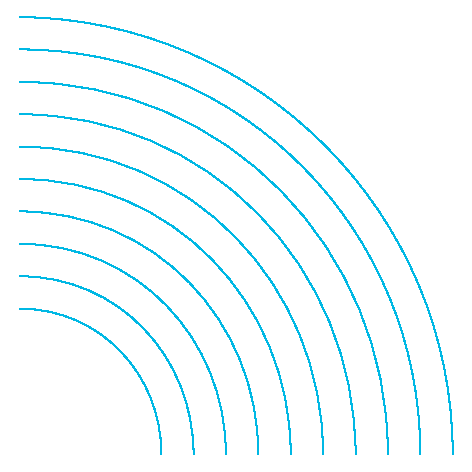
\includegraphics[width=.15\paperwidth,height=.15\paperwidth]{EETtemplateFiles/img/Simbolo_ESCOLA.pdf}\\
  
\includegraphics[width=.15\paperwidth,trim={.4cm .5cm .4cm 2.25cm},clip]{EETtemplateFiles/img/Logotipo_ESCOLA.pdf}
  \vspace*{-11pt}%
}

% MATH SYMBOLS

\newcommand{\field}[1]{\mathbb{#1}}

\DeclareMathOperator{\atan}{atan}
\DeclareMathOperator{\acos}{acos}
\DeclareMathOperator{\asin}{asin}

% \newcommand{\mb}[1]{\mathbf{#1}}


\newcommand{\Hb}{\mathbf{H}}
\newcommand{\Sb}{\mathbf{\boldsymbol{\Sigma}}}
\newcommand{\Sm}{\mathbf{S}}
\newcommand{\U}{\mathbf{U}}
\newcommand{\F}{\mathbf{F}}
\newcommand{\V}{\mathbf{V}}
\newcommand{\A}{\mathbf{A}}
\newcommand{\B}{\mathbf{B}}
\newcommand{\Cb}{\mathbf{C}}
\newcommand{\D}{\mathbf{D}}
% \newcommand{\E}{\mathbf{E}}
\newcommand{\Gb}{\mathbf{G}}
\newcommand{\T}{\mathbf{T}}
\newcommand{\I}{\mathbf{I}}
\newcommand{\Y}{\mathbf{Y}}
\newcommand{\M}{\mathbf{M}}
\newcommand{\N}{\mathbf{N}}
\newcommand{\W}{\mathbf{W}}
\newcommand{\Z}{\mathbf{Z}}
\newcommand{\R}{\mathbf{R}}
\newcommand{\K}{\mathbf{K}}
\newcommand{\X}{\mathbf{X}}
\newcommand{\Pb}{\mathbf{P}}
\newcommand{\Lb}{\mathbf{L}}
\newcommand{\Phib}{\mathbf{\boldsymbol{\Phi}}}
\newcommand{\Upsb}{\mathbf{\boldsymbol{\Upsilon}}}
\newcommand{\Delb}{\mathbf{\boldsymbol{\Delta}}}
\newcommand{\Xib}{\mathbf{\boldsymbol{\Xi}}}
\newcommand{\Q}{\mathbf{Q}}
% \newcommand{\D}{\mathbf{D}}
\newcommand{\one}{\mathbf{1}}
\newcommand{\zero}{\mathbf{0}}
\newcommand{\Rm}{\mathbf{R^{-1}}}
\newcommand{\LL}{\mathbf{\boldsymbol{\Lambda}}}
\newcommand{\J}{\mathbf{J}}

\newcommand{\ab}{\mathbf{a}}
\newcommand{\bb}{\mathbf{b}}
\newcommand{\cc}{\mathbf{c}}
\newcommand{\dd}{\mathbf{d}}
\newcommand{\e}{\mathbf{e}}
\newcommand{\f}{\mathbf{f}}
\newcommand{\g}{\mathbf{g}}
\newcommand{\h}{\mathbf{h}}
\newcommand{\m}{\mathbf{m}}
\newcommand{\n}{\mathbf{n}}
\newcommand{\pp}{\mathbf{p}}
\newcommand{\q}{\mathbf{q}}
\newcommand{\rr}{\mathbf{r}}
\newcommand{\s}{\mathbf{s}}
\newcommand{\uu}{\mathbf{u}}
\newcommand{\vv}{\mathbf{v}}
\newcommand{\w}{\mathbf{w}}
\newcommand{\x}{\mathbf{x}}
\newcommand{\y}{\mathbf{y}}
\newcommand{\z}{\mathbf{z}}
\newcommand{\al}{\mathbf{\boldsymbol{\alpha}}}
\newcommand{\vmu}{\mathbf{\boldsymbol{\mu}}}
\newcommand{\vlambda}{\mathbf{\boldsymbol{\lambda}}}
\newcommand{\vphi}{\mathbf{\boldsymbol{\phi}}}
\newcommand{\vrho}{\mathbf{\boldsymbol{\rho}}}
\newcommand{\vups}{\mathbf{\boldsymbol{\upsilon}}}

\newcommand{\rank}{\textnormal{rank}}
% \newcommand{\trace}{\textnormal{trace}}
\newcommand{\exptr}{\textnormal{exptr}}
\newcommand{\tr}{\textnormal{tr}}
\newcommand{\vstack}{\textnormal{vec}}
\newcommand{\diag}{\textnormal{diag}}
%  |x>
\newcommand{\ket}[1]{\left\vert#1\right\rangle}
%  <x|
\newcommand{\bra}[1]{\left\langle#1\right\vert}
%  <x|y>
\newcommand{\braket}[2]{\left< #1 \vphantom{#2}\,
                        \right\vert\left.\!\vphantom{#1} #2 \right>}
%  <x|a|y>
\newcommand{\sandwich}[3]{\left< #1 \vphantom{#2 #3} \right|
                          #2 \min\left(\vphantom{#1 #2} #3 \right>}

\newcommand{\pd}[2]{\frac{\partial #1}{\partial #2}}
%  d/dt
\newcommand{\ddt}{\frac{d}{dt}}
%  D/Dx
\newcommand{\pdd}[1]{\frac{\partial}{\partial#1}}
%  |x|
\newcommand{\abs}[1]{\left\vert#1\right\vert}
%  k_{x}
\newcommand{\kv}[1]{\mathbf{k}_{#1}}
%  \textnormal{E}_{domain of integration}{variable}
\newcommand{\Ex}[2]{{\mathbb{E}_{#1}\left[#2\right]}}
\newcommand{\CEx}[3]{{\mathbb{E}_{#1}\left[#2|#3\right]}}
\newcommand{\CInf}[3]{{\textnormal{I}\left(#1;#2|#3\right)}}
\newcommand{\Inf}[2]{{\textnormal{I}\left(#1;#2\right)}}
\newcommand{\CEnt}[2]{{\textnormal{H}\left(#1|#2\right)}}
\newcommand{\Ent}[1]{{\textnormal{H}\left(#1\right)}}
\newcommand{\dCEnt}[2]{{\textnormal{h}\left(#1|#2\right)}}
\newcommand{\dEnt}[1]{{\textnormal{h}\left(#1\right)}}

\newcommand{\cmark}{\ding{51}}%
\newcommand{\xmark}{\ding{55}}%
\newcommand\Tau{\mathcal{T}}
%Figure and format fixes


\renewcommand{\figurename}{Fig.}
\newcommand{\PESrule}{\noindent\rule{.57\columnwidth}{0.1mm}}

% A command to make itemized table contents

%theroem environments
% If using amsthm package, we need to delete these theorems before giving them our own definition. does not work for theorem
% \let\theorem\relax
\let\definition\relax
\let\lemma\relax
\let\corollary\relax
\let\example\relax
%
% \newtheorem{theorem}{Theorem}
\newtheorem{definition}{Definition}
\newtheorem{lemma}{Lemma}
\newtheorem{corollary}{Corollary}
\newtheorem{conjecture}{Conjecture}
\newtheorem{example}{Example}
\theoremstyle{plain}
\newtheorem{remark}{Remark}
\newtheorem{proposition}{Proposition}
   \newtheorem{homework}{Homework}

%Colors
   \definecolor{blueH3}{rgb}{0,.5,1}
   \definecolor{blueH2}{rgb}{0,0.25,0.75}
   \definecolor{blueH1}{rgb}{0,0,0.5}   
   \definecolor{grayOldText}{rgb}{.5,.5,.5}
   \definecolor{VCobalt}{HTML}{005682}
   \definecolor{TZTeal}{HTML}{008080}
   \definecolor{TZTealfaded}{HTML}{F0FFFF}
   \definecolor{KYJade}{HTML}{008151}
   \definecolor{ARust}{HTML}{a10000}
   \definecolor{FFucsia}{HTML}{7000c3}   
   \definecolor{TAMustard}{HTML}{a1a100}
   \definecolor{Tangerine}{HTML}{d45500}
   
   %%%%%%%%%%%%%%%%%%%%%%%%%%%%%%%%%%%%%%%%%%%%%%%%%%%%%%%%%%%%%%%%%
%% The following definitions are to extend the LaTeX algorithmic 
%% package with SWITCH statements and one-line structures.
%% The extension is by 
%%   Prof. Farn Wang 
%%   Dept. of Electrical Engineering, 
%%   National Taiwan University. 
%% 
\newcommand{\SWITCH}[1]{\STATE \textbf{switch} (#1)}
\newcommand{\ENDSWITCH}{\STATE \textbf{end switch}}
\newcommand{\CASE}[1]{\STATE \textbf{case} #1\textbf{:} \begin{ALC@g}}
\newcommand{\ENDCASE}{\end{ALC@g}}
\newcommand{\CASELINE}[1]{\STATE \textbf{case} #1\textbf{:} }
\newcommand{\DEFAULT}{\STATE \textbf{default:} \begin{ALC@g}}
\newcommand{\ENDDEFAULT}{\end{ALC@g}}
\newcommand{\DEFAULTLINE}[1]{\STATE \textbf{default:} }
%% 
%% End of the LaTeX algorithmic package extension.

\newcounter{MYtempeqncnt}


%%%%%%%%%%%%%%%%%%%%%%%%%%%%%%%%%%%%%%%
% Commands to recall text later
%%%%%%%%%%%%%%%%%%%%%%%%%%%%%%%%%%%%%%%
\makeatletter
\newcommand\remembertext[2]{% #1 is a key, #2 is the text
  \immediate\write\@auxout{\unexpanded{\global\long\@namedef{mytext@#1}{#2}}}%
  #2%
}
%
\newcommand\recalltext[1]{%
  \ifcsname mytext@#1\endcsname
    \@nameuse{mytext@#1}%
  \else
    ``??''
  \fi
}

%%%%%%%%%%%%%%%%%%%%%%%%%%%%%%%%%%%%%%%%%%%%%%%%%%%%%%%%%%%%%%%%%%%%%%%%%%%%%%%%%%
%%% Paolo Casari: macros for automating section titling and comment formatting %%%
%%%%%%%%%%%%%%%%%%%%%%%%%%%%%%%%%%%%%%%%%%%%%%%%%%%%%%%%%%%%%%%%%%%%%%%%%%%%%%%%%%
\newcounter{myequationcnt}

\newcounter{rcnt}
\newcounter{ccnt}

\newcommand{\newreviewernopagebreak}[1]{\vspace{5em} \setcounter{ccnt}{0}\section*{\normalsize Comments of #1}\vspace{4mm}}

\newcommand{\ThisIsTheEditorNoPageBreak}{\setcounter{ccnt}{0}\section*{\Large Comments of the Editor}\vspace{3mm}}
\newcommand{\ThisIsTheEditor}{\clearpage \ThisIsTheEditorNoPageBreak}
\newcommand{\ThisIsANewReviewerNoPageBreak}[1]{\vspace{5em} \refstepcounter{rcnt}\label{r#1}\setcounter{ccnt}{0}\section*{\Large Comments of Reviewer \arabic{rcnt}}\vspace{3mm}}
\newcommand{\ThisIsANewReviewer}[1]{\clearpage\vspace{-5em} \ThisIsANewReviewerNoPageBreak{#1}}

\newcommand{\edcomment}[1]{
\begin{tcbremark}
\color{VCobalt}
    \refstepcounter{ccnt}\label{e\arabic{ccnt}}\noindent\textbf{\boldmath\emph{Comment E.\arabic{ccnt}:}} #1\vspace{0.2cm}
\end{tcbremark}
}
\newcommand{\refedcomment}[1]{E.\ref{e#1}}

\newcommand{\revcomment}[1]{
\begin{tcbremark}
\color{VCobalt}
\refstepcounter{ccnt}\label{r\arabic{rcnt}c\arabic{ccnt}}\noindent\textbf{\boldmath\emph{Comment \arabic{rcnt}.\arabic{ccnt}:}} #1\vspace{0.2cm}
\end{tcbremark}
}
\newcommand{\refrevcomment}[2]{\ref{r#1}.\ref{r#1c#2}}

% \newcommand{\ouranswer}[1]{\noindent\emph{Answer:} #1\vspace{0.6cm}}
% \newcommand{\citepap}[1]{\vspace{0.33cm}\begin{minipage}{0.05\textwidth} $\phantom{A}$  \end{minipage}\begin{minipage}{0.85\textwidth}\renewcommand{\baselinestretch}{1.15}\small \emph{#1} \end{minipage}\vspace{0.3cm}}

\newlength{\ansspace}
\addtolength{\ansspace}{0.6cm}
\newcommand{\ansbreak}{\vspace{\ansspace}}

\newlength{\stdleftskip}
\addtolength{\stdleftskip}{\leftskip}
\newlength{\stdrightskip}
\addtolength{\stdrightskip}{\rightskip}
\newlength{\citeskip}
\addtolength{\citeskip}{2em}
\newcommand{\oldbaselinestretch}{1.5}

\newcommand{\setcitepapskip}{%
    \leftskip\citeskip %
    \rightskip\citeskip %
    \renewcommand{\baselinestretch}{1.15}\small%
    \vspace{0.6em}%
    \noindent%
}

\newcommand{\resetLRmargins}{%
    \leftskip\stdleftskip %
    \rightskip\stdrightskip %
    \renewcommand{\baselinestretch}{\oldbaselinestretch}\normalsize %
    \vspace{0.6em}
}

\newcommand{\emans}{\emph{Answer:\ }}


%---------------
% LIMIAR
%---------------
%configuracion de opcions de beamer persoais, pero alleas ao estilo

% COMANDO QUE INTRODUCE UNHA DIAPOSITIVA CUN ÍNDICE NO QUE APARECEN VELADAS TÓDALAS SECCIÓNS MENOS A ACTUAL. ÚTIL PARA INTRODUCIR OS TÍPICOS ÍNDICES INTERMEDIOS.
\newcommand{\Inter}{\frame{\tableofcontents[currentsection]}}
\newcommand{\inter}{\frame{\tableofcontents[currentsection,currentsubsection]}}

% Pes de imaxe
\renewcommand{\figurename}{Fig.}
\addto\captionsenglish{\renewcommand{\figurename}{Fig.}}
\setbeamertemplate{caption}[numbered]

%ESTE PAQUETE PERMITE POÑER A BIBLIOGRAFIA AO PE DE PAXINA CON CONFIGURACIONS ESTETICAS PERSOAIS
% \usepackage[style=ieee,doi=false,isbn=false,url=true,backend=bibtex]{biblatex}
% \bibliography{./bibliografia.bib}
% \newrobustcmd*{\footfullcitenomark}{%
%   \AtNextCite{%
%     \let\thefootnote\relax 
%     \let\mkbibfootnote\mkbibfootnotetext
%     }%
%   \footfullcite}

%paquete para engadir notas de guion ao pdf
\usepackage{pgfpages}
% \setbeameroption{show only notes} 
% \setbeameroption{show notes}
% \setbeameroption{show notes on second screen=right}
% DATOS DO DOCUMENTO
\title{Advanced Communication Systems}
\subtitle{Part 2.4:\\ Multi-user Communications:\\ Medium Access Protocols}
\author[FGC]{Felipe G\'omez Cuba}
\institute[XX]{
\begin{columns}[T]
\begin{column}{9cm}\centering
Despacho 204\\
Titorías: Lun-Xov 15:00-16:30\\
(En caso de confinamento: videochamada a calquera horario acordado)\\
  \texttt{gomezcuba@gts.uvigo.es}\\
\end{column}
\end{columns}
}

\date{17 \& 19 November 2020 }

\begin{document}

% Diapositiva co título
%\frame[plain]{\titlepage}%the ``classic'' beamer cover pageç

\frame{\frametitle{\\}%generate top bar, but blank line as tittle
\titlepage
}%approximation to the ``GPSC ppt'' cover page, but with central beamer title

% \frame{\tableofcontents}
% \note[itemize]{%itemized notes are special ``note'' slides that beamer can append to the pdf or not, depending on a boolean toggle option
% \item Introduce yourself
% \item In this work we studied blablabla.
% }

% \section{IAB MmWave Network}

\frame[allowframebreaks]{\frametitle{Classification of Access Schemes}

\begin{itemize}
 \item Fixed Assignment Schemes
    \begin{itemize}
        \item Suitable for fixed rate applications
        \item Examples: FM Radio, TV, Satellite TV...
        \item Old mobile voice TDMA/FDMA/CDMA (long time scale)\\ \ \\
    \end{itemize}
 \item Dynamic Assignment Schemes
    \begin{itemize}
        \item Managed by a \textbf{scheduler} (centralized)
        \item Rapid variation in allocations
        \item OFDMA or TDMA/FDMA (fast time scale)\\ \ \\
    \end{itemize}
 \item Contention-based Schemes
    \begin{itemize}
        \item Users choose attempt instant (distributed)
        \item Attempts to use channel may fail
        \item Random but regulated\\ \ \\ 
    \end{itemize}
\end{itemize}

}


\frame[allowframebreaks]{\frametitle{Dynamic Allocation}

\begin{itemize}
 \item In a real system, data is generated at random intervals
 \begin{itemize}
    \item A web request ($\sim$Bytes) starts a download (kB-MB)
    \item A video stream sends a frame every $\sim 20$ms
    \item Smart meters may send only 32 bit every 15 minutes\\ \ \\
 \end{itemize}
 
 \item Dynamic resource allocation can ``look for'' good channel\\ \ \\
 \item Main difference between Fixed and Dynamic contention-free schemes is adaptation to traffic and channel state
    \begin{figure}    
    \setcounter{subfigure}{0}
    \subfigure[Fixed allocation problems]{
    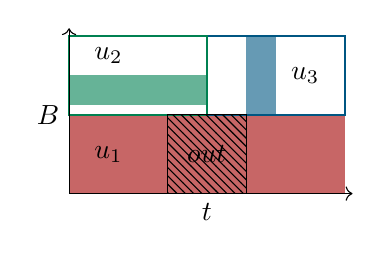
\begin{tikzpicture}[scale=.25]
        \fill[color=ARust!60,thick] (0,0) rectangle (14,4);
        \fill[color=VCobalt!60] (9,4) rectangle (10.5,8);
        \fill[color=KYJade!60] (0,4.5) rectangle (7,6);
        \draw[color=VCobalt,thick] (7,4) rectangle (14,8);
        \draw[color=KYJade,thick] (0,4) rectangle (7,8);
        \draw[pattern=north west lines, pattern color=black] (5,0) rectangle (9,4);
%         \draw[help lines,color=black,dashed] (0,0) grid (14,8);   
        \draw [->] (0,0) -- (0,8.4);
        \draw [->] (0,0) -- (14.4,0);
        \node [anchor=center] at (2,2) {$u_1$};
        \node [anchor=center] at (2,7) {$u_2$};
        \node [anchor=center] at (12,6) {$u_3$};
        \node [anchor=center] at (7,2) {$out$};
        \node [anchor=north] at (7,0) {$t$};
        \node [anchor=east] at (0,4) {$B$};         
    \end{tikzpicture}
    }
    \subfigure[OFDMA Dynamic Scheme]{
            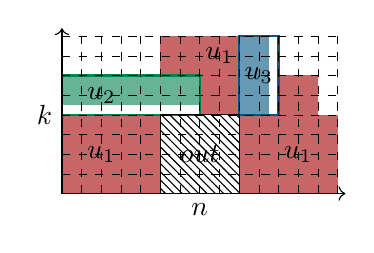
\begin{tikzpicture}[scale=.25]
            \fill[color=VCobalt!60] (9,4) rectangle (10.5,8);
            \fill[color=KYJade!60] (0,4.5) rectangle (7,6);
                \fill[color=ARust!60] (0,0) rectangle (5,4);
                \fill[color=ARust!60] (9,0) rectangle (14,4);
                \fill[color=ARust!60] (9,0) rectangle (14,4);
                \fill[color=ARust!60] (5,6) rectangle (9,8);
                \fill[color=ARust!60] (7,4) rectangle (9,6);
                \fill[color=ARust!60] (7,4) rectangle (9,6);
                \fill[color=ARust!60] (11,4) rectangle (13,6);
            \draw[color=VCobalt,thick] (9,4) rectangle (11,8);
            \draw[color=KYJade,thick] (0,4) rectangle (7,6);
                \draw[help lines,color=black,dashed] (0,0) grid (14,8); 
        \draw[pattern=north west lines, pattern color=black] (5,0) rectangle (9,4);  
        \node [anchor=center] at (7,2) {$out$};
                \draw [->] (0,0) -- (0,8.4);
                \draw [->] (0,0) -- (14.4,0);
                \node [anchor=center] at (2,2) {$u_1$};
                \node [anchor=center] at (8,7) {$u_1$};
                \node [anchor=center] at (12,2) {$u_1$};
                \node [anchor=center] at (2,5) {$u_2$};
                \node [anchor=center] at (10,6) {$u_3$};
                \node [anchor=north] at (7,0) {$n$};
                \node [anchor=east] at (0,4) {$k$};         
            \end{tikzpicture}
    }
    \end{figure}
\vspace{-.5in}
\end{itemize}



}

\frame[allowframebreaks]{\frametitle{Multi-user Diversity}

\begin{definition}[OFDMA Scheduling Algorithms]
 A central entity (BS usually) knows the traffic needs of all users for the next \textit{frame} of $N$ consecutive OFDM sysmbols and selects which user is assigned to each \textit{Resource Block} with index $[n,k]$.
\end{definition}
\ \\
\begin{itemize}
 \item Round Robin Scheduler: Each user gets $\frac{1}{K}$ resources in order\\ \ \\
 \item Max-Throughput Scheduler: Each resource $[n,k]$ user with \textbf{best channel} is assigned
    $\arg\max_u|h_{u}[n,k]|^2$
    \begin{itemize}
        \item \textbf{Fair} if $P_u$'s equal and $h_{u}[n,k]$'s i.i.d.
        \item \textbf{Starvation} with unequal channels
        \item Maximum sum rate
        $$\Ex{}{\frac{B}{K}\log\left(1+\frac{P_u}{BN_o}\max_u\{|h_{u}|^2\}\right)}\geq\Ex{}{\frac{B}{K}\log\left(1+\frac{P_u}{BN_o}|h_{u}|^2\right)}$$
    \end{itemize}
    
   \pagebreak
   \item Denote the instantaneous SNR as $\rho_u=\frac{P}{BN_o}|h_u|^2$\\ \ \\
   \item Define the normalization $\overline{\rho}_u=\frac{\rho_u}{\Ex{}{\rho_u}}=\frac{|h_{u}|^2}{\Ex{}{|h_{u}|^2}}$\\ \ \\

   \item Proportional Fair Scheduler: $\arg\max_u\overline{\rho}_u$
    \begin{itemize}
        \item Always fair ($P(\overline{\rho}_u=\overline{\rho}_{\max})=\frac{1}{K}$ in Rayleigh)\\ \ \\
        \item Some Multiuser Diversity $\Ex{}{\overline{\rho}_u|\overline{\rho}_u=\overline{\rho}_{\max}}>\Ex{}{\overline{\rho}_u}$\\ \ \\
        \item Not Maximum Throughput ($\Ex{}{\max \overline{\rho}_{u}}\leq\frac{\Ex{}{\max \rho_u}}{\Ex{}{\rho_u}}$)\\ \ \\
    \end{itemize}
   \item PF achieves more sum-rate than RR without losing fairness, but sacrificing \textbf{delay}
\end{itemize}
}


\frame[allowframebreaks]{\frametitle{Joint SDMA+OFDMA}
    \begin{itemize}
     \item Capacity of MAC and BC achieved by non-orthogonal schemes\\ \ \\
     \item Exploitation of MIMO to increase DoF of the wireless system\\ \ \\
     \item Scheduler in 3D: time, frequency and antenna port $[n,k,p]$ \\ \ \\
    \begin{figure}
            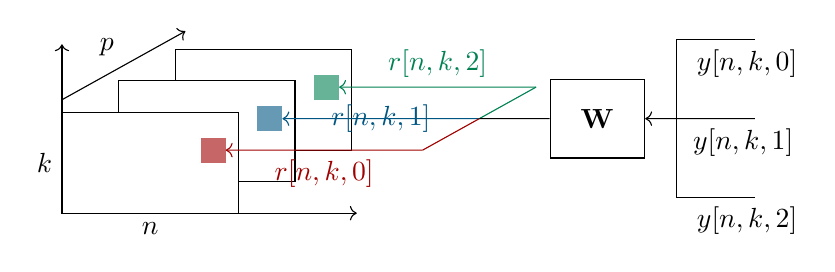
\begin{tikzpicture}[scale=.16]
                \fill[color=white] (9,5) rectangle (23,13); 
                \draw[color=black] (9,5) rectangle (23,13); 
                \fill[color=white] (4.5,2.5) rectangle (18.5,10.5); 
                \draw[color=black] (4.5,2.5) rectangle (18.5,10.5); 
                \fill[color=white] (0,0) rectangle (14,8); 
                \draw[color=black] (0,0) rectangle (14,8); 
                \draw [->] (0,0) -- (0,13.4);
                \draw [->] (0,0) -- (23.4,0);
                \draw [->] (0,9) -- node [anchor=south east] {$p$} (9.8,14+.8*5/9);
                \node [anchor=north] at (7,0) {$n$};
                \node [anchor=east] at (0,4) {$k$};   
                \fill[color=ARust!60] (11,4) rectangle (13,6);   
                \fill[color=VCobalt!60] (15.5,6.5) rectangle (17.5,8.5);   
                \fill[color=KYJade!60] (20,9) rectangle (22,11);  
                \node[input] (grapheast1) at (13,5) {};
                \node[input] (grapheast2) at (17.5,7.5) {};
                \node[input] (grapheast3) at (22,10) {}; 
                \coordinate[right of=grapheast3,node distance = 2.5cm] (prefilt3); 
                \coordinate[right of=grapheast2,node distance = 2.5cm] (prefilt2);  
                \coordinate[right of=grapheast1,node distance = 2.5cm] (prefilt1);  
                \node[block,right of=prefilt2,node distance = 1.5cm] (filt) {$\W$};  
                \coordinate[right of=filt,node distance = 1cm] (posfilt);  
                \node[output,right of=posfilt,node distance=1cm] (ant2) {};
                \node[output,above of=ant2,node distance=1cm] (ant1) {};
                \node[output,below of=ant2,node distance=1cm] (ant3) {};
                \draw [draw,<-,color=ARust] (grapheast1) -- node[anchor=north,pos=.5]{$r[n,k,0]$} (prefilt1);
                \draw [draw,<-,color=VCobalt] (grapheast2) -- node[anchor=center,pos=.5]{$r[n,k,1]$} (prefilt2);
                \draw [draw,<-,color=KYJade] (grapheast3) -- node[anchor=south,pos=.5]{$r[n,k,2]$} (prefilt3);
                \draw [draw,-,color=KYJade] (prefilt3) --  (prefilt2);
                \draw [draw,-,color=ARust] (prefilt1) -- (prefilt2);
                \draw [draw] (prefilt2) -- (filt);
                \draw [draw,<-] (filt) -- (posfilt);
                \draw [draw] (posfilt) |- node[anchor=north,pos=.95 ]{$y[n,k,0]$} (ant1);
                \draw [draw] (posfilt) -- node[anchor=north,pos=.85 ]{$y[n,k,1]$} (ant2);
                \draw [draw] (posfilt) |- node[anchor=north,pos=.95 ]{$y[n,k,2]$} (ant3);
            \end{tikzpicture}
            
    \caption{OFDMA+SDMA receiver with linear filter $\W$}
    \end{figure}
    \pagebreak
    \item Users assigned same time-frequency RB $\mathcal{A}[n,k]\subset \{1,2,\dots U\}$\\ \ \\
    \item Let $\Hb_{\mathcal{A}}=\left(\h_{a(1)},\h_{a(2)},\dots \h_{a(N_{ant})}\right)$\\ \ \\
    \item Matched filter $\Hb_{\mathcal{A}}^H$ asymptotically optimal for $\h_i^H\h_j\approx 0$ \\ \ \\
    \item We can simplify the MAC receiver/BC transmitter a lot by grouping users that are ``physically'' orthogonal by luck\\ \ \\
    \end{itemize}
}
\frame[allowframebreaks]{\frametitle{\small Homework: Boolean Non-Convex Scheduling Optimization}

% \begin{homework}
Consider a MAC with 4 single-antenna transmitters. The receiver has 2 antennas and performs a TDMA subdivision of users in 2 groups of 2 users denoted $\mathcal{A}$ and $\mathcal{B}$. The resulting DEC is
$$\y[n]=\begin{cases}
        \sum_{i\in \mathcal{A}}\h_ix_i[n]+\z[n]&\textnormal{for even }n\\
        \sum_{i\in \mathcal{B}}\h_ix_i[n]+\z[n]&\textnormal{for odd }n\\
       \end{cases}
$$
If we define the boolean vector $\bb$ with $b_i=1$ if user $i$ is in group $\mathcal{B}$, and $b_i=0$ if user $i$ is in group $\mathcal{A}$, the DEC can also be written as 
$$\y[n]=\begin{cases}
        \Hb(\I-\LL_\bb)\x[n]+\z[n]&\textnormal{for even }n\\
         \Hb\LL_\bb\x[n]+\z[n]&\textnormal{for odd }n\\
       \end{cases}
$$
where $\Hb$ contains all the four column channel vectors, and $\LL_{\bb}$ is a diagonal matrix with $\bb$ in its diagonal. 
% \end{homework}

\textit{Assume the transmitters have power $P$ and the receiver knows $\bb$ and employs a bank of MMSE filters $\w_i=\h_i^H(\Hb_{eff}\Hb_{eff}^H+\frac{\sigma^2}{P}\I)^{-1}$ where $\Hb_{eff}=\Hb(\I-\LL_\bb)$ or $\Hb_{eff}=\Hb\LL_\bb$ depending on $n$.}
\begin{enumerate}
 \item \textit{Write the SINRs and rates of each user $i$ depending on $b_i$, $\LL_\bb$, $\w_i$, $\Hb$, etc.}
 \item \textit{Using all the rates above, write a ``maximum-sum-rate'' scheduling problem to choose $\bb$}
 
 \textit{(you \textbf{do not} have to solve the optimization, just formulate it. hint: for all groups of two $\sum b_i=2$)}
\end{enumerate}
}

\frame[allowframebreaks]{\frametitle{Machine to Machine Communications}
    
\begin{itemize}
 \item Connectivity for small devices
 \begin{itemize}
    \item Farming / forest fire / intruder alarm sensors
    \item Smart electric grid / city streets / cars / healthcare
    \item Payment / Parking / Toll / ``Vending'' terminals
    \item etc.\\ \ \\
 \end{itemize}
 \item Battery and hardware complexity limitations\\ \ \\
 \item Large number of users in large area range\\ \ \\

 \item Very short messages
 \begin{definition}[Control Overhead]
  The ratio $\frac{L_{message}}{L_{control}+L_{message}}$ represents rate waste. Typically random schemes with very low $L_{control}$ are preferable when $L_{message}$ is small.
 \end{definition}
\end{itemize}
}

\frame[allowframebreaks]{\frametitle{ALOHA}
 \begin{itemize}
  \item First wireless data packet network, Uni. of Hawaii, 1971\\ \ \\
  \item Each user tries to transmit when data arrives\\ \ \\
  \item If transmissions collide, random repeat timer $\textnormal{Exp}(\beta)$
 
 \begin{definition}[Poisson Arrival Process]
  An infinite number of users uniformly distributed in an infinite space with density $\lambda$. Ordered $\dots T_{i-1}<T_{i}<T_{i+1}\dots$
  $$\lim_{K\to\infty} \left\{T_k\sim\textnormal{Unif}\left(-\frac{1}{2\lambda K},\frac{1}{2\lambda K}\right)\right\}^K\sim \textnormal{PAP}(\lambda) $$
 \end{definition}

    \begin{figure}
            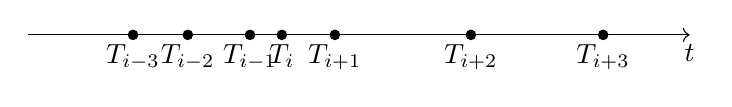
\begin{tikzpicture}[scale=.6]
            \draw[->] (0,0) -- (14,0);
            \node[anchor=north] at (14,0) {$t$};
            
            \coordinate (pos0) at (2.218012163873324,0);
            \coordinate (pos1) at (3.377484394358655,0);
            \coordinate (pos2) at (4.69382170479299,0);
            \coordinate (pos3) at (5.36784707364627,0);
            \coordinate (pos4) at (6.489585361893921,0);
%             \coordinate (pos5) at (9.096856047292288,0);
%             \coordinate (pos6) at (9.13638337192597,0);
%             \coordinate (pos7) at (9.277688782289555,0);
            \coordinate (pos5) at (9.368839240196047,0);
            \coordinate (pos6) at (12.168294610137748],0);
            \foreach \x in {0,...,6}{%            
                \draw[fill=black] (pos\x) circle (.1);
                \pgfmathparse{int(\x-3)}ç
                \ifthenelse{\pgfmathresult>0}{
                    \node[anchor=north] at (pos\x) {$T_{i+\pgfmathresult}$};
                    }
                    {
                    \ifthenelse{\pgfmathresult=0}{
                        \node[anchor=north] at (pos\x) {$T_{i}$};
                        }
                        {
                        \node[anchor=north] at (pos\x) {$T_{i\pgfmathresult}$};
                        }
                    }
            }
            \end{tikzpicture}
    \end{figure}
  \pagebreak
  \item No. arrivals in a time interval $\Phi(\Delta T)\sim \textnormal{Poisson}(k,\lambda\Delta T)$\\ \ \\
  \item Inter-arrival time $\Upsilon_i=T_{i}-T_{i-1} \sim \textnormal{Exp}(\lambda)$\\ \ \\
  \item Memoryless $P(\Upsilon_i>x|\Upsilon_i>\xi)=P(\Upsilon_i>x-\xi)$\\ \ \\
  \begin{columns}
   \begin{column}{5cm}
    \item Arrivals with $n$ retrans. waiting 
        $$G(n)=(\lambda+n\beta)\tau_{msg}$$
    \item Success probability 
        $$P(\Phi(2\tau_{msg})=0)=e^{-2G(n)}$$
        
    \begin{figure}
            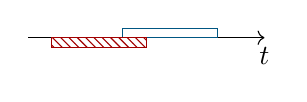
\begin{tikzpicture}[scale=.6]
            \draw[->] (2,0) -- (7,0);
            \node[anchor=north] at (7,0) {$t$};
            \draw[color=VCobalt] (4,0) rectangle (6,.2);
            \draw[color=ARust,pattern=north west lines, pattern color=ARust] (2.5,0) rectangle (4.5,-.2);
            \end{tikzpicture}
    \end{figure}
   \end{column}
   \begin{column}{5cm}
    \item ALOHA efficiency 
        $$S(G(n)) = G(n)e^{-2G(n)}\leq 18\%$$
    \begin{figure}
            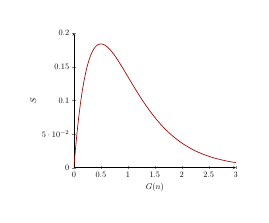
\begin{tikzpicture}[scale=.3]
       \begin{axis}[
            axis lines = left,
            xlabel = $G(n)$,
            ylabel = {$S$},
            ymax=.2,
%             legend style={at={(.95,.53)}}
        ]
        \addplot [thick,
            domain=0:3, 
            samples=100, 
            color=ARust,
        ]
        {x*exp(-2*x)};
        \end{axis}
            \end{tikzpicture}
    \end{figure}
   \end{column}

  \end{columns}  
  \vspace{-.5in}
 \end{itemize}
}


\frame[allowframebreaks]{\frametitle{Classic Contention-Based Schemes}
\begin{itemize}
 \item Slotted ALOHA
 \begin{itemize}
  \item Transmission start synchronization
  \item Removes $\frac{1}{2}$ collision interval ($35\%$ ef.)
  
  
    \begin{figure}
        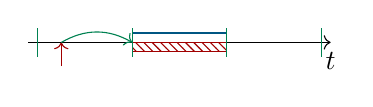
\begin{tikzpicture}[scale=.6]
        \draw[->] (1.8,0) -- (8.2,0);
        \node[anchor=north] at (8.2,0) {$t$};
        \draw[color=VCobalt] (4,0) rectangle (6,.2);
        \draw[color=ARust,pattern=north west lines, pattern color=ARust] (4,0) rectangle (6,-.2);
        \draw[->,color=ARust] (2.5,-.5) -- (2.5,0);
        \draw[->,color=KYJade] (2.5,0) to [out=30,in=150] (4,0);
        \foreach \x in {1,2,...,4}{
            \draw[color=KYJade] (2*\x,-.3) -- (2*\x,.3);
        }
        \end{tikzpicture}
    \end{figure}
  
 \end{itemize}
 \item CSMA/CD (old coax. ethernet):
    \begin{itemize}
        \item ``Listen before/while talk''
        \item Minimal collision interval $\propto$ propagation\\ \ \\
    \end{itemize}
 \item Token-Pass: No collisions, turns instead\\ \ \\
 \item CSMA/CA (WiFi):
    \begin{itemize}
        \item Random tx. timer after ``listening'' to free channel
        \item Virtual Carrier Sensing (RTS/CTS)\\ \ \\
    \end{itemize}
\end{itemize}
}

\frame[allowframebreaks]{\frametitle{ALOHA-based M2M Satellite Systems}
 \begin{itemize}
    \item Satellite: very long delay and power limitations    
    \begin{itemize}
        \item Delay $\to$ No CS, retransmissions very damaging
        \item \textbf{Very low load ALOHA to achieve packet loss $<10^{-3}$}\\ \ \\
    \end{itemize}
    \item Diversity Slotted ALOHA:
    \begin{itemize}
        \item Two copies to reduce delay (no RTT wait)
        \item Capture: Decode stronger user in collision
            \begin{figure}
            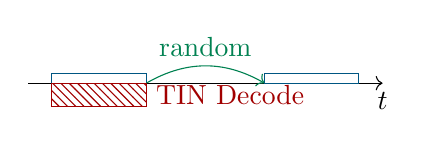
\begin{tikzpicture}[scale=.6]
            \draw[->] (3.5,0) -- (11,0);
            \node[anchor=north] at (11,0) {$t$};
            \draw[color=VCobalt] (4,0) rectangle (6,.2);
            \draw[color=VCobalt] (8.5,0) rectangle (10.5,.2);
            \draw[->,color=KYJade] (6,0) to [out=30,in=150] node[anchor=south,color=KYJade] {random} (8.5,0);
            \draw[color=ARust,pattern=north west lines, pattern color=ARust] (4,0) rectangle (6,-.5);
            \node[color=ARust,anchor=west] at (6,-.25) {TIN Decode};
            \end{tikzpicture}
    \end{figure}
    \end{itemize}
    \item Spread Spectrum ALOHA:
    \begin{itemize}
        \item Better than SA/DSA with equal power
        \item Poor performance under power inbalance 
    \end{itemize}
    \pagebreak
    \item Contention Resolution Diversity SA:
        \begin{itemize}
            \item Each replica contains control info with time-position of copies
            \item After successful decoding $\to$ SIC of past collisions
            \begin{figure}
            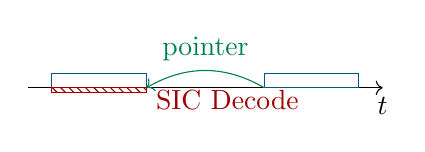
\begin{tikzpicture}[scale=.6]
            \draw[->] (3.5,0) -- (11,0);
            \node[anchor=north] at (11,0) {$t$};
            \draw[color=VCobalt] (4,0) rectangle (6,.3);
            \draw[color=VCobalt] (8.5,0) rectangle (10.5,.3);
            \draw[->,color=KYJade] (8.5,0) to [out=150,in=30] node[anchor=south,color=KYJade] {pointer} (6,0);
            \draw[color=ARust,pattern=north west lines, pattern color=ARust] (4,0) rectangle (6,-.1);
            \node[color=ARust,anchor=west] at (6,-.25) {SIC Decode};
            \end{tikzpicture}
    \end{figure}
 \end{itemize}
    \item Coded Random Access (a.k.a. Irregular Repetition SA)
    \begin{itemize}
       \item N users with activation prob. $p_a$
       \item Random number of replicas $d$ with prob. $P(d)$
       \item Random instants over $S$ slots, ${S \choose d}$
       \item If \textit{logical load} $G=\frac{p_aN}{S}<G^{th}\to P(\textnormal{SIC success})\approx 1$
       \item Random $d$ no significant advantage over CRDSA\\ \ \\
    \end{itemize}
    \item Enhanced SSA / MMSE E-SSA:
    \begin{itemize}
       \item Asynchronous, desirable in SatCom
       \item SSA with iterative SIC / and MMSE
    \end{itemize}
 \end{itemize}
}


\frame[allowframebreaks]{\frametitle{Low Power Wide Area Networks (LPWAN)}
\begin{itemize}
 \item Massive long-range low-rate low-power devices (M2M)\\ \ \\
 \item LoRaWAN
 \begin{columns}
  \begin{column}{2cm} 
 \begin{figure}  
  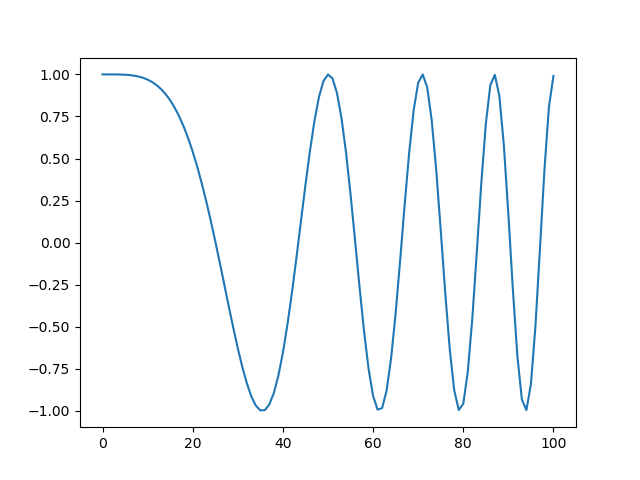
\includegraphics[width=\columnwidth]{chirp}
 \end{figure}  
  \end{column}
  \begin{column}{12cm}
 \begin{itemize}
 \item Propietary LoRa modulation (Chirp Spread Spectrum)
 \item Very robust to narrowband interference 
\end{itemize}
  \end{column}
 \end{columns}
 \item SigFox
    \begin{itemize}
    \item Very low rate DBPSK with random $f_c$ and time instant $\times 3$
    \item Ultra Narrow Band (UNB): change of $f_c$ > $B$\\ \ \\
    \end{itemize}
 \item 3GPP NB-IoT
    \begin{itemize}
        \item Subset of LTE with reduced complexity
        \item Subcarrier scheduling with 200kHz bandwidth
    \end{itemize}
\end{itemize}


}
\frame[allowframebreaks]{\frametitle{Superposed Contention and Scheduling}
\begin{itemize}
 \item Ultra Reliable Low Latency Communications (URLLC) in 5G\\ \ \\
 \item Coexistence in the same network
 \begin{itemize}
    \item \textbf{Low-rate} critical services (hospitals, military etc.)
    \item High-demand delay-resistent mobile broadband\\ \ \\
\end{itemize}
 \item MBB RB allocations can be stolen
    \begin{itemize}
    \item URLLC transmit when they want, \textbf{capture} RBs
    \item MBB signal can recover from on/off interference
    \item Works if URLLC traffic $\ll$ MBB traffic
    \end{itemize}
    
\begin{figure}    
            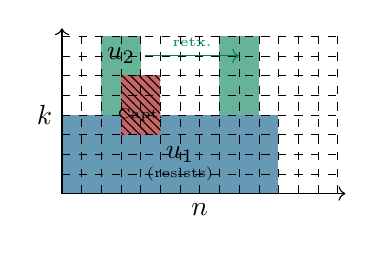
\begin{tikzpicture}[scale=.25]
                \fill[color=VCobalt!60] (0,0) rectangle (11,4);
                \fill[color=KYJade!60] (2,4) rectangle (4,8);
                \fill[color=ARust!60] (3,3) rectangle (5,6);
                \fill[pattern=north west lines, pattern color=black] (3,3) rectangle (5,6);
                \fill[color=KYJade!60] (8,4) rectangle (10,8);
                \draw[help lines,color=black,dashed] (0,0) grid (14,8); 
                \node [anchor=center] at (4,4) {\tiny Capt.};
                \draw [->] (0,0) -- (0,8.4);
                \draw [->] (0,0) -- (14.4,0);
                \node [anchor=north] at (7,0) {$n$};
                \node [anchor=east] at (0,4) {$k$};   
                \node [anchor=center] at (6,2) {$u_1$};
                \node [anchor=center] (u2) at (3,7) {$u_2$};
                \draw[->,color=KYJade] (u2) to node[anchor=south] {\tiny retx.} (9,7);   
                \node [anchor=center] at (6,1) {\tiny (resists)};
            \end{tikzpicture}
    \end{figure}
\end{itemize}

}
\end{document}


